\subsection{Dallamszerkesztés az akkord vertikális értelmezésével}
\label{sec:exdallamvert}
Szerkesszünk dallamot A-dúr hangnemben, a hangnem akkordjainak kíséretére!
\begin{pitemize}
Funkció & T & ST(SD) & M(D,T) & SD & D & SM(SD,T) & V(D) \\ \hline
Az skála hangjai & A & H & \cisz & D & E & \fisz & \gisz \\
Hármashangzatai & $A$ & $H_m$ & $C^\#_m$ & $D$ & $E$ & $F^\#_m$ & $G^{\#\dim}$ \\
Négyeshangzatai & $A^{maj7}$ & $H_m^7$ & $C^{\#7}_m$ & $D^{maj7}$ & $E^{7}$ & $F^{\#7}_m$ & $G^{\#\sdim7}$ \\ 
\end{pitemize}
Horizontális felfogásban a skála akkordjait a skála hangjaiból álló dallam kíséri.
Hogy egy kicsit érdekesebben hangozzék, két ütemen keresztül a funkciót vertikálisan értelmezzük.
A következő lépés azon skálák meghatározása, melyekben az általunk kiválasztott kísérő akkordok szerepelnek. Ezúttal legyen ez a domináns $E^7$.
Vizsgáljuk meg a fokokról induló akkordok típusait a ,,\nameref{sec:skalaakkordok}'' mellékletben. \\\\
A melodikus moll skála negyedik fokán, a kulcshangtól kvart távolságra elhelyezkedő 
$E^{7}$-hez a hangközfordítás szabályai szerint a kulcshang E-től tiszta kvint távolságra van,
tehát a keresett skála az $H_m$:
H, \cisz, D, E, \fisz, \gisz, \aisz. \\\\
A melodikus moll skála ötödik fokán, a kulcshangtól kvint távolságra elhelyezkedő 
$E^{7}$-hez a hangközfordítás szabályai szerint a kulcshang E-től tiszta kvart távolságra van,
tehát a keresett skála az $A_m$:
A, H, C, D, E, \fisz, \gisz. \\\\
A harmonikus moll skála ötödik fokán, a kulcshangtól kvint távolságra elhelyezkedő 
$E^{7}$-hez a hangközfordítás szabályai szerint a kulcshang E-től tiszta kvart távolságra van,
tehát a keresett skála az $A_m$:
A, H, C, D, E, F, \gisz. \\\\
Az utolsó kettőből és az alapskálából alkotott kilenc fokú alterált skála:
A, H, C, \cisz, D, E, F, \fisz, \gisz \\\\
Pillér hangok $E^7$-hez:
E, \gisz, H, D \\\\
Diatonikus váltóhangok (a kísérő akkord hangjait elhagyva):
A, C, \cisz, F, \fisz \\\\
Kromatikus váltóhangok:
(E pillérhanghoz) \disz,
(\gisz pillérhanghoz) G, \aisz,
(H pillérhanghoz) \aisz,
(D pillérhanghoz) \disz. \\\\
Az első öt ütem horizontális értelmezés szerint a skála hangjaival kísért akkordokat tartalmaz. A következő kettő érdekesebben hangzik: a dallammenet  E - \aisz - H - D, \gisz - F - H - \gisz. Szerkezete PH - KV - PH - PH, PH - DV - PH - PH. 

\begin{figure}[!htbp]
 \advance\leftskip-6mm
 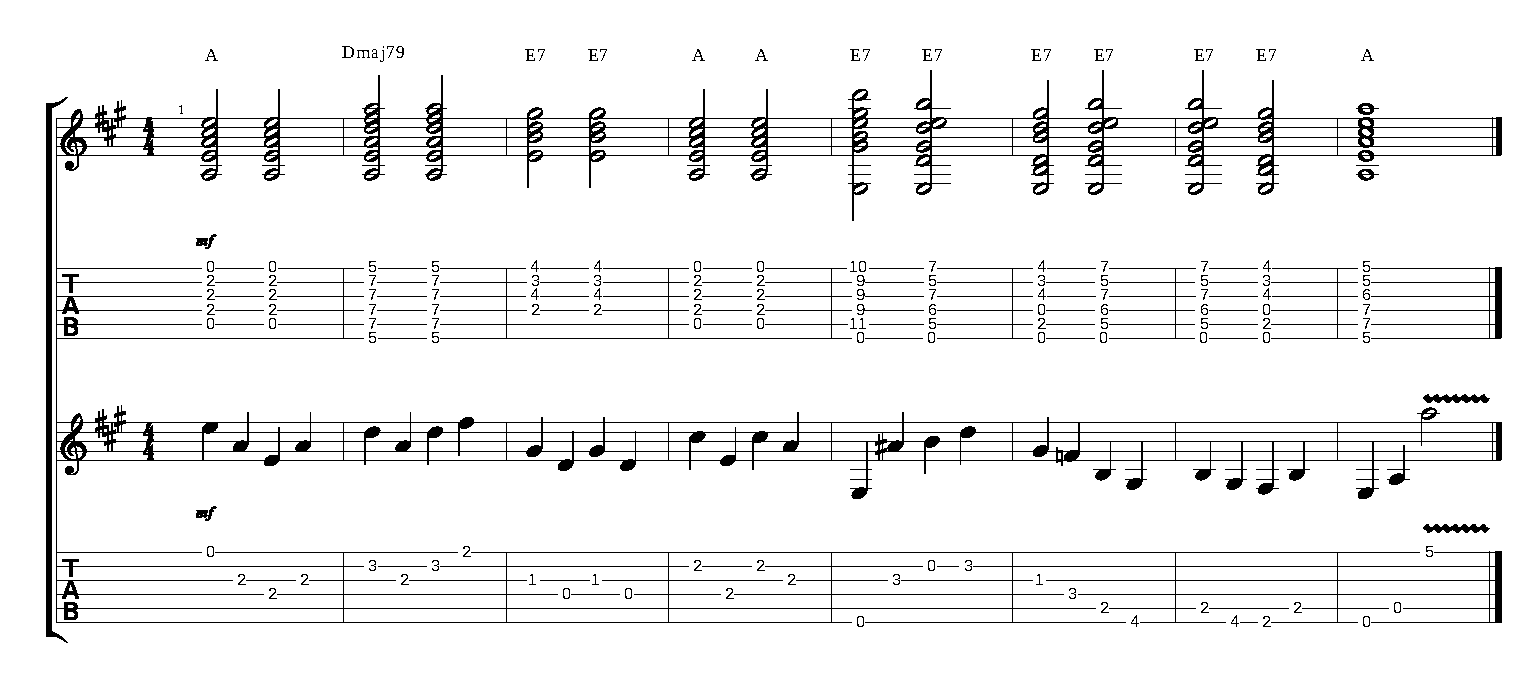
\includegraphics[page=1,scale=0.70]{notes/dallamszerkesztes.pdf}
\end{figure}

\subsection{Dallamszerkesztés enharmonikus kiegészítéssel}
\label{sec:exdallamenharm}
Az előbbi példában leírt akkord kíséretre most írjunk dallamot az $E^7$ akkord enharmonikusaihoz tartozó skálákból! \\\\
$E$, \textcolor{red}{\gisz, $H$ és $D$} $\longrightarrow$ \gisz\ignorespaces$^\dim$ \\
\textcolor{red}{$H$ és $D$} + \fisz $\longrightarrow$ $H_m$ \\
\textcolor{red}{$H$ és $D$} + $F$ $\longrightarrow$ $H^O$ \\
\cisz + \textcolor{red}{$E$ és \gisz} $\longrightarrow$ \cisz$_m$ \\
$C$ + \textcolor{red}{$E$ és \gisz} $\longrightarrow$ $C^+$ \\
$A$, \cisz + \textcolor{red}{$E$ és \gisz} $\longrightarrow$ $A^{maj7}$ (A-dúr skála) \\
\aisz, \cisz + \textcolor{red}{$E$ és \gisz} $\longrightarrow$ $A^{\#\sdim}$ \\
\textcolor{red}{\gisz, $H$}, $D$ $\longrightarrow$ \gisz$_m$ \\
$A$, $C$, \textcolor{red}{$E$, \gisz} $\longrightarrow$ $A_m/^{maj7}$ (A-moll skála) \\\\
A fenti lehetőségek közül válasszuk a \cisz$_m$ és az $A$ skálákat - ezek uniója: $E$, \fisz, \gisz, $A$, $H$, $C$, \cisz, $D$, \disz. Az ötödik, hatodik és hetedik ütemben ennek a skálának a hangjait használjuk, ügyelve arra, hogy az első és a harmadik ütem pillér hanggal kezdődjön:
 
\begin{figure}[!htbp]
 \advance\leftskip-6mm
 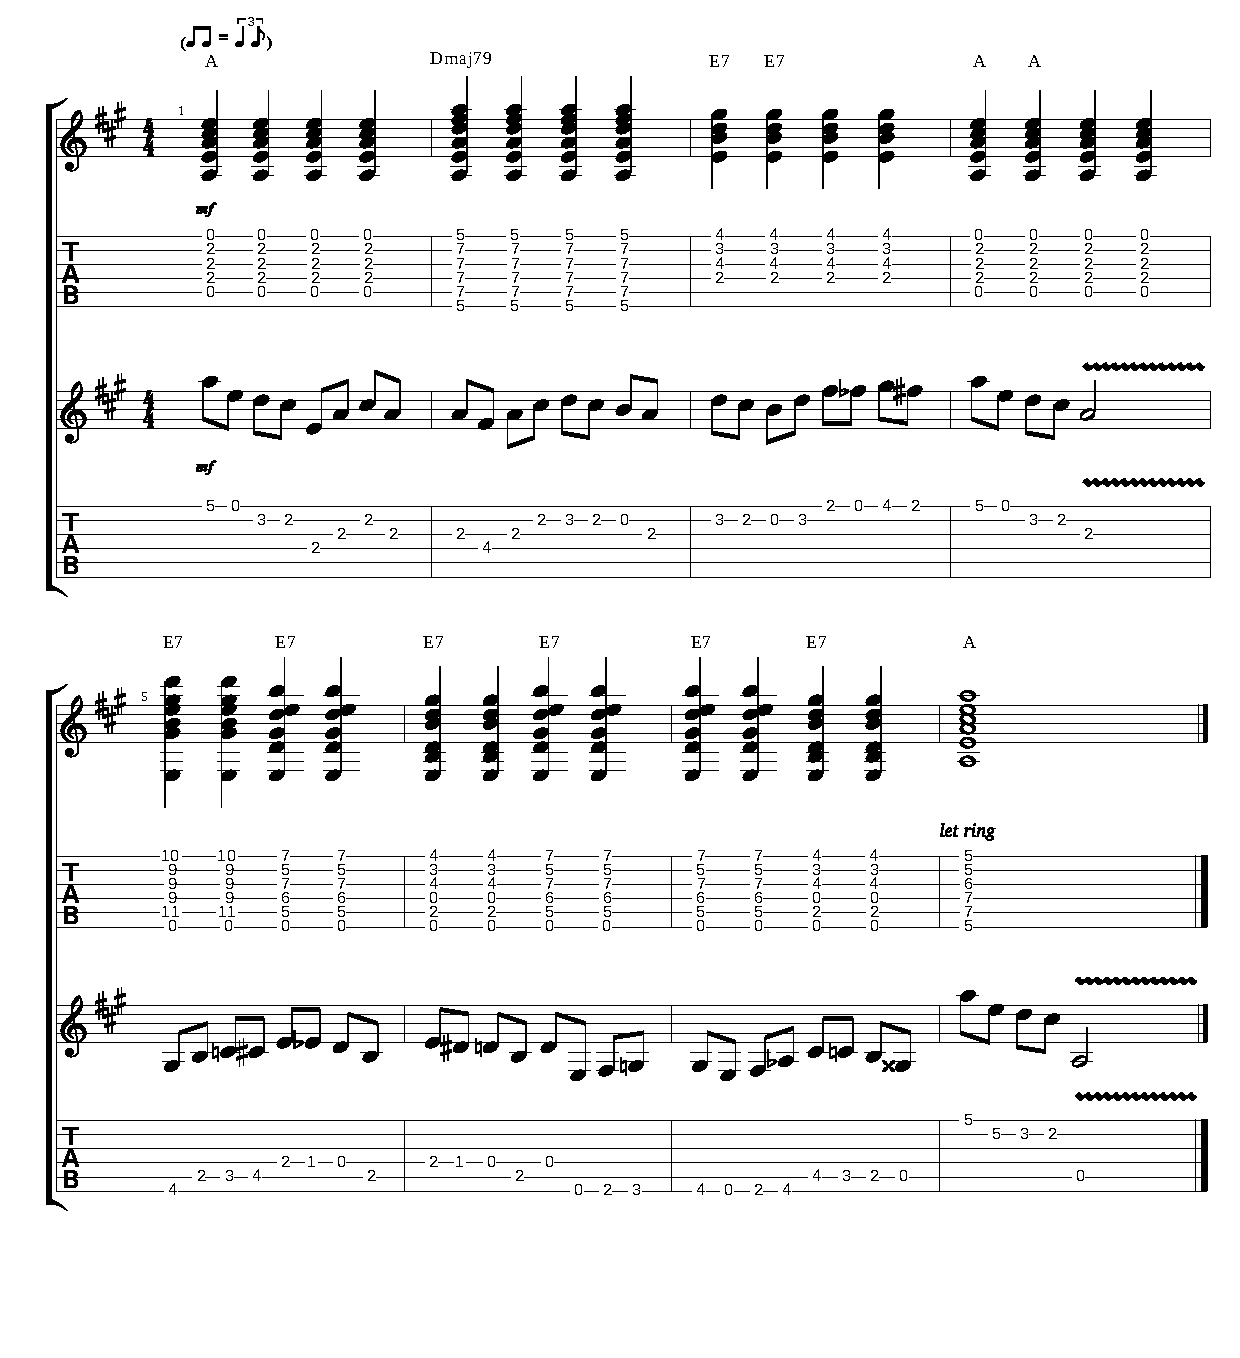
\includegraphics[page=1,scale=0.85]{notes/dallamszerkesztes_II.pdf}
\end{figure}
